\documentclass[./main.tex]{subfiles}

\begin{document}
\section{Finetuning}
\label{sec:finetuning}
As we now have pretrained our models, we need to finetune the models, such that they are specialized to yield optimial results on the ClimbAlong dataset. The following section describes the finetuning of these models. This includes the preprocessing of the data, the configuration details we use, as well as the obtained results.
\\
\\
In the finetuning stage we will be using the keypoint detector to train our temporal-inclusive models. However, we will be freezing the pose detector, such that the weights of the model will not change during the training and we will thus only train our temporal-inclusive models. We do this as (1) the training of the models will be quicker, as we just need to train the temporal-inclusive models and not the keypoint detector, and (2) we get an greater understanding of the effects of our models when combined with the pose detector, as we can clearly see how big of a difference it makes by adding our temporal-inclusive models.
\\
\\
In section \ref{sec:finetune_data_preprocessing} we cover the preprocessing of the finetune dataset. Then, in section \ref{sec:pretrain_details} we cover the used configuration for the finetuning. Then, in section \ref{subsec:finetune_train_val_res} and section \ref{subsec:finetune_test_res} we cover the training and validation results, as well as the testing results, respectively. Lastly, in section \ref{sec:finetune_tech_details} we cover the technical details of the finetuning.

\subsection{Data Preprocessing}
\label{sec:finetune_data_preprocessing}
For the ClimbAlong dataset we perform only minor preprocessing. First, the preprocessing of each video is done by having the keypoint detector process the video, such that we have the output heatmaps of the pose detector, containing all of the pose-estimations of each video. Next, we preprocess the heatmaps by setting all negative values to $0$ and normalizing each heatmap, such that each heatmap sums up to the fixed value $c = 255$ that we used when preprocessing the BRACE and Penn Action datasets, essentially making the heatmaps more similar to the preprocessed heatmaps of BRACE and Penn Action. These heatmaps will then be used as the input for our models.
\\
\\
For the ground truth heatmaps we create twenty five heatmaps of each frame, similarly to how we did it for the BRACE and Penn Action datasets, however, in this case we use the predicted bounding-box of the pose detector as our bounding-box. In cases where the ground truth keypoint is placed outside of the bounding-box, we place the ground truth keypoint at the closest border of the bounding-box.

\subsection{Training Details}
\label{sec:pretrain_details}
\begin{figure}[htbp]
    \centering
    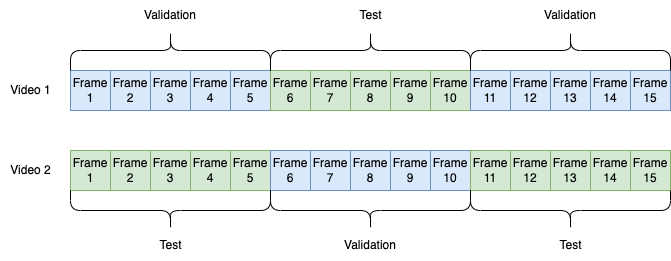
\includegraphics[width=0.8\textwidth]{entities/CA_splitting.png}
    \caption{Illustration of how the ClimbAlong data has been split into a validation dataset and a test dataset.}
    \label{fig:CA_splitting}
\end{figure}
\noindent \textbf{Data Configuration} Generally, for the data configuration we follow a similar approach to how we did in the pretraining stage. We again use a window-size of $k = 5$ frames, resulting in a total of $10,173$ windows. Also here are we using $c = 255$ as a representation of the ground truth placement of each keypoint. 
\\
\\
As this dataset is much smaller than the dataset used during the pretraining-stage, we can much more easily introduce some evaluation-bias, hence why we also take much more careful steps. Thus, the splitting of the dataset is different than how we performed it in the pretraining-stage. First, we extract the longest video, such that none of its windows are on the dataset, which we will use to ensure, that our validation and testing of our models is unbiased. Next, we use the first $60\%$ of frame-windows of the remaining part of the dataset and use those as the training dataset. For the other $40\%$ of the frame-windows, we make sure that they have no overlapping frames the with training dataset, as these windows will be used for evaluating the models. If they do have any overlapping frames with the training dataset, the whole window is moved into the training dataset. As we still have to split the remaining $40\%$ of the frame-windows into a validation dataset and a test dataset, we have to make sure, that (1) both datasets use as many video sequences as possible, which is especially important in this case due to the small dataset size, (2) that none of the windows are overlapping between the two datasets, and (3) both datasets sample the windows uniformly distributed throughout the video sequences, as there can be some sepcial movements in certain parts of the video sequences. All of these constraints will make sure that we minimize the evaluation-bias of our models. The splitting of the remaining $40\%$ of the window into two datasets is then done by sorting the non-overlapping windows by their video and by their time of occurence in their corresponding video. Then, if the $i$th window-frame is divisible by two, it is moved into the validation dataset, otherwise it is moved into the test dataset. By doing so we meet all three of our conditions. The overall idea has been illustrated in Figure \ref{fig:CA_splitting}.
\\
\\
\textbf{Experiments} As the finetuning dataset is very small, the fitting of the models are very quick, making us fit all of the 26 developed models from the pretraining stage, instead of us picking which models we should finetune. For each model we pick the epoch from the pretraining stage, that yielded the highest validation PCK@0.2 accuracy and use that for finetuning.
\\
\\
\textbf{Training Configuration} The optimization parameters are very similar to the ones from the pretraining stage. We again use the MSE loss-function, a batch size of $16$, and the ADAM optimizer with $\rho_1 = 0.9$ and $\rho_{2} = 0.999$ as these two values were suggested by \cite{DL_book}. During training, we again keep track of the lowest reached validation loss of an epoch and use learning rate reduction and early-stopping in a similar manner to how we did in the pretraining stage. However, unlike the pretraining stage, we here use a smaller initial learning rate of $10^{-4}$, as the weights only need to be fineadjusted, making us believe that a greater learning rate would skew the weights too much.

\subsection{Training and Validation Results}
\label{subsec:finetune_train_val_res}
\begin{figure}[htbp]
    \centering
     \begin{subfigure}[b]{\textwidth}
         \centering
         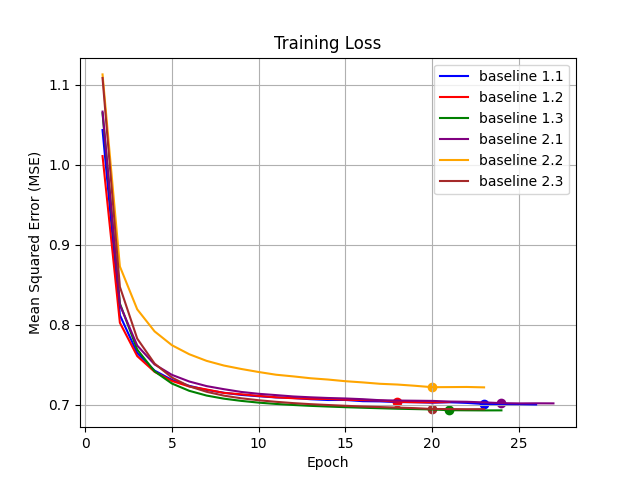
\includegraphics[width=0.32\textwidth]{./entities/finetuned/baseline/train_losses.png}
         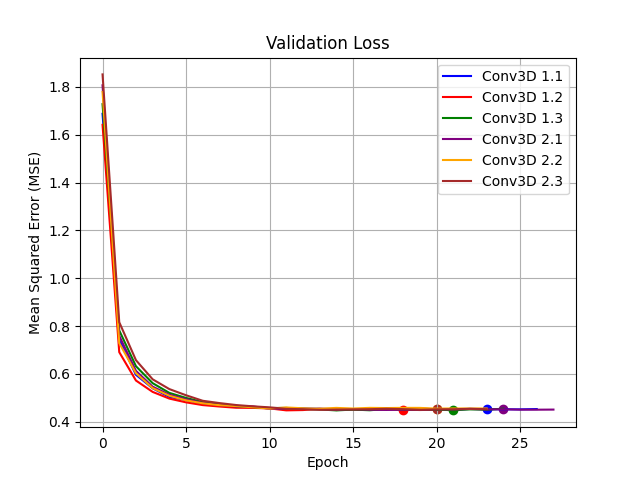
\includegraphics[width=0.32\textwidth]{./entities/finetuned/baseline/val_losses.png}
         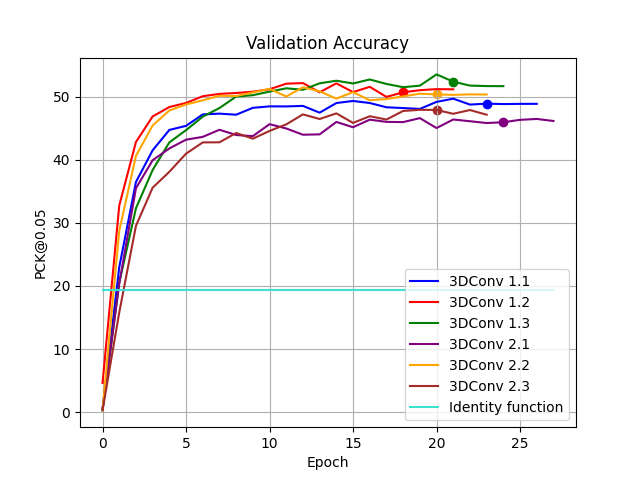
\includegraphics[width=0.32\textwidth]{./entities/finetuned/baseline/val_accs.png}
         \caption{Finetuning results of 3DConv.}
     \end{subfigure}
    \hfill

    \begin{subfigure}[b]{\textwidth}
        \centering
        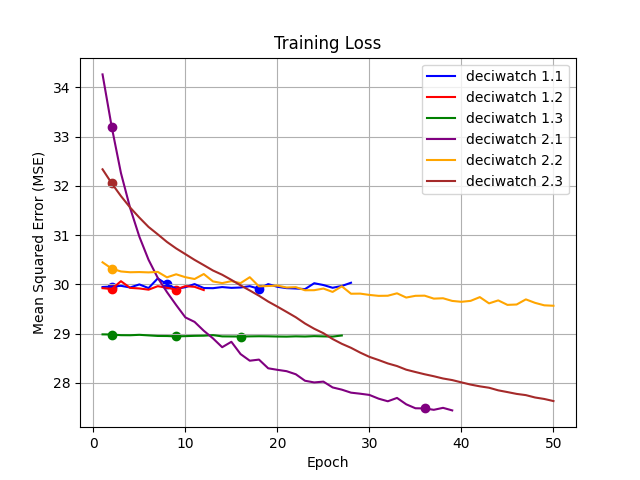
\includegraphics[width=0.32\textwidth]{./entities/finetuned/deciwatch/train_losses.png}
        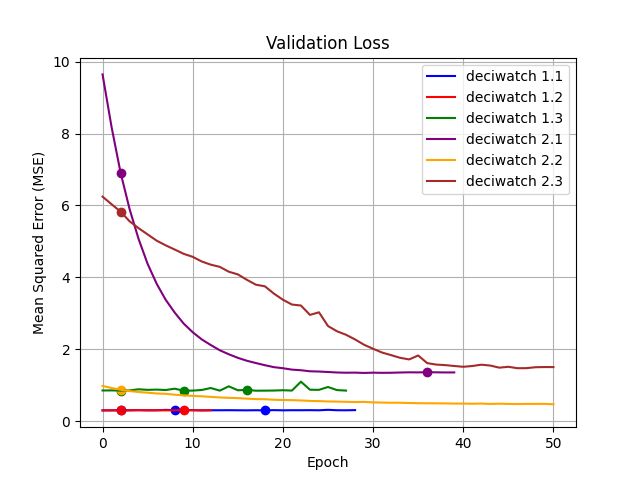
\includegraphics[width=0.32\textwidth]{./entities/finetuned/deciwatch/val_losses.png}
        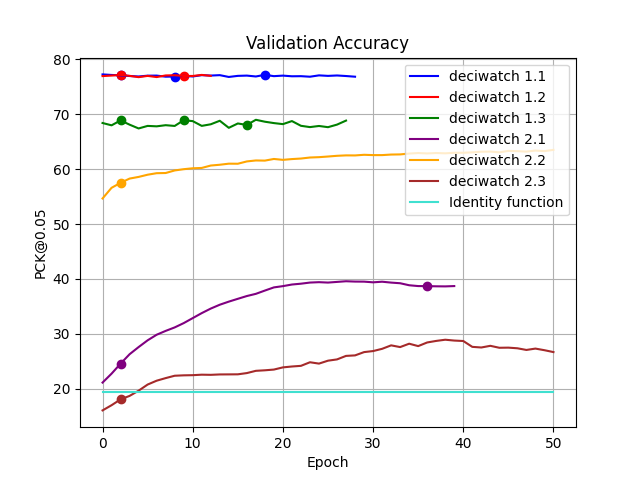
\includegraphics[width=0.32\textwidth]{./entities/finetuned/deciwatch/val_accs.png}
        \caption{Finetuning results of DeciWatch.}
    \end{subfigure}
   \hfill

   \begin{subfigure}[b]{\textwidth}
    \centering
    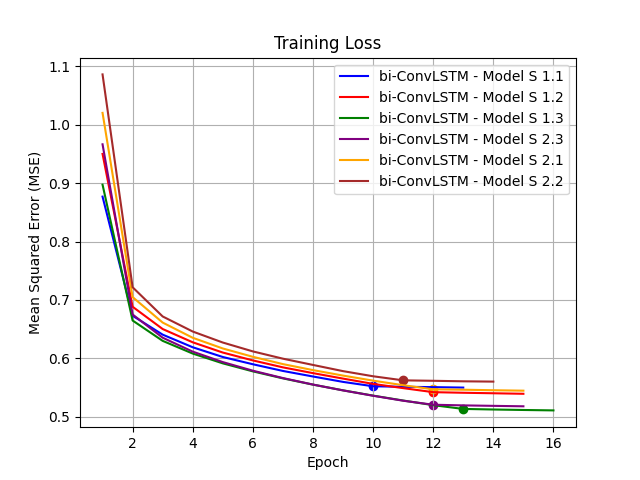
\includegraphics[width=0.32\textwidth]{./entities/finetuned/unipose/train_losses.png}
    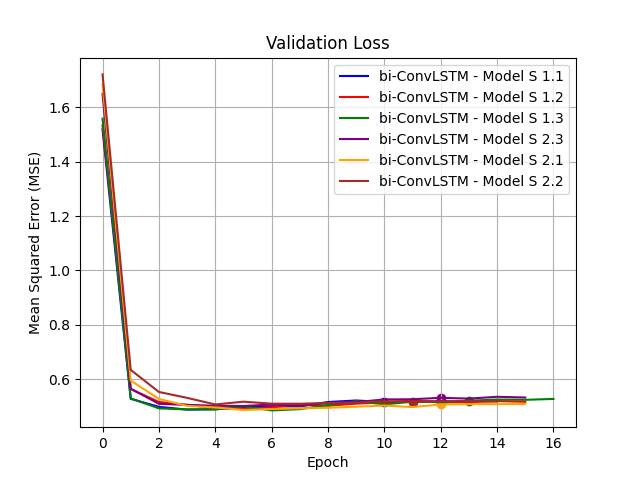
\includegraphics[width=0.32\textwidth]{./entities/finetuned/unipose/val_losses.png}
    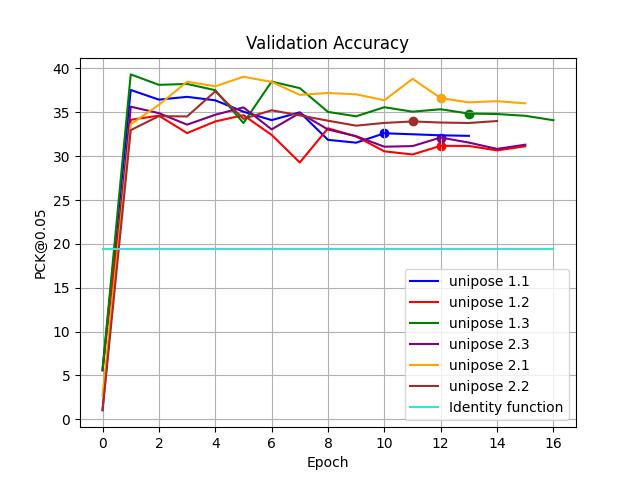
\includegraphics[width=0.32\textwidth]{./entities/finetuned/unipose/val_accs.png}
    \caption{Finetuning results of bi-Conv LSTM Model S.}
    \end{subfigure}
    \hfill

    \begin{subfigure}[b]{\textwidth}
        \centering
        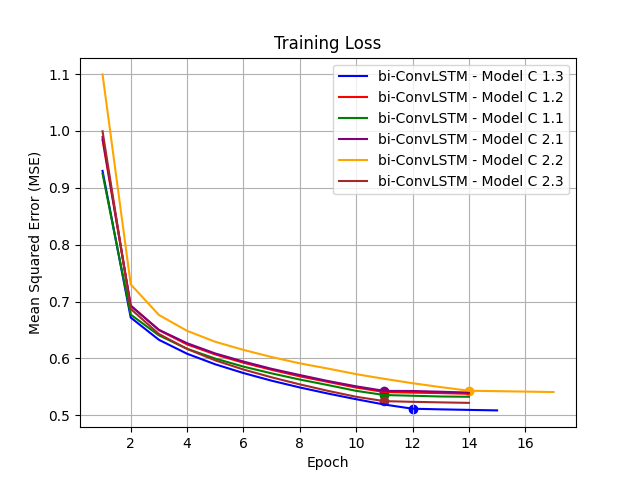
\includegraphics[width=0.32\textwidth]{./entities/finetuned/unipose2/train_losses.png}
        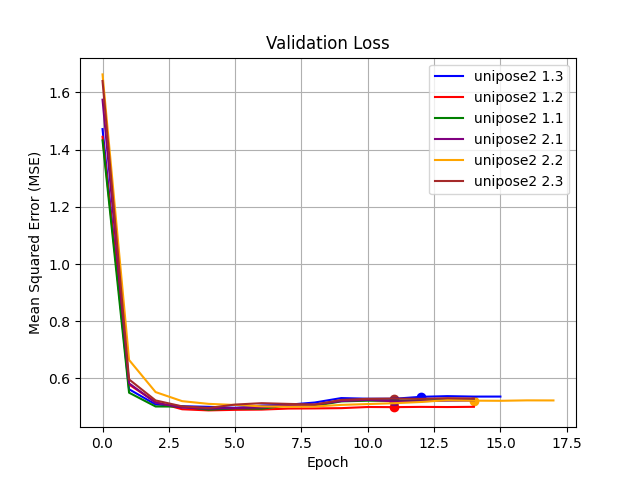
\includegraphics[width=0.32\textwidth]{./entities/finetuned/unipose2/val_losses.png}
        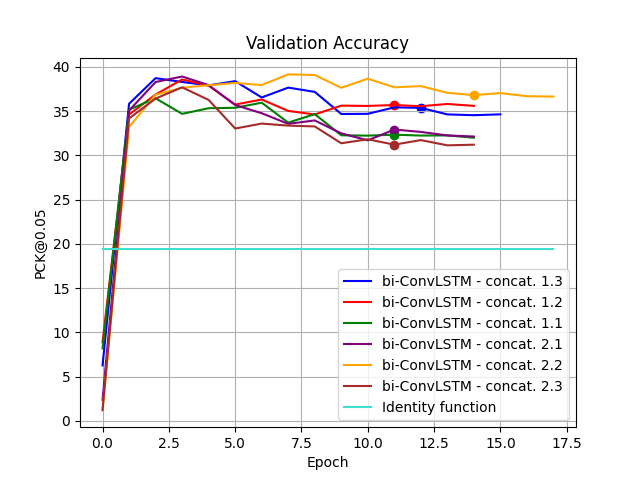
\includegraphics[width=0.32\textwidth]{./entities/finetuned/unipose2/val_accs.png}
        \caption{Finetuning results of bi-Conv LSTM Model C.}
    \end{subfigure}
    \hfill
    
    \caption{Evolution of the training loss, validation loss and validation PCK@0.05 accuracy of the 24 models during training, as well as the validation PCK@0.05 accuracy of the identity function of the two datasets. The dots indicates a reduction of learning rate. First row: 3DConv. Second row: DeciWatch. Third row: Finetuning results of bi-Conv LSTM Model S. Fourth row: Finetuning results of bi-Conv LSTM Model C.}
    \label{fig:finetune_res}
\end{figure}

We have in Figure \ref{fig:finetune_res} illustrated the evaluation of the training loss, validation loss, and validation PCK@0.05 accuracy of the various models during the finetuning.
\\
\\
If we compare the models against the identity function we clearly see, how all models at some point beats the identity function, indicating the positive effects of incorporating temporal information into pose estimation.
\\
\\
Generally, 3DConv seems to be converging towards the greatest results, as these models tend to converge towards the highest validation PCK@0.05 accuracy. However, some DeciWatch runs actually starts off with an even higher validation PCK@0.05 accuracy, which then decreases to a much lower value quickly. The two architectures that are based on a bidirectional convolutional LSTM tend to yield some decent results, however, their training tend to plateau rather early, hence why they also terminate very quickly. Generally however, both DeciWatch and the two architectures based on a bidirectional convolutional LSTM do seem to overfit. For DeciWatch this is mostly immediately, whereas for the bidirectional convolutional LSTMs this tend to happen a few epochs later.
\\
\\
Further, the shifting-scalar seems to only have a minor effect on the models during the finetuning, as all six runs of each model tend converge towards the same result.

\subsubsection{Additional Experiment Results}
\label{sec:finetune_additional_experiment}
\begin{figure}
    \centering
    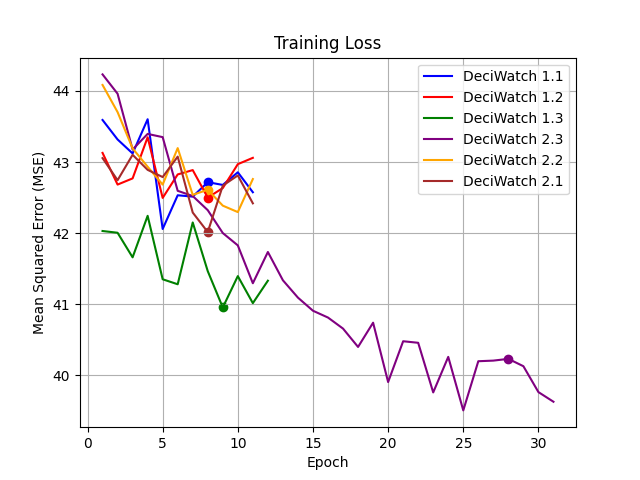
\includegraphics[width=0.32\textwidth]{./entities/finetuned/adapted/train_losses.png}
    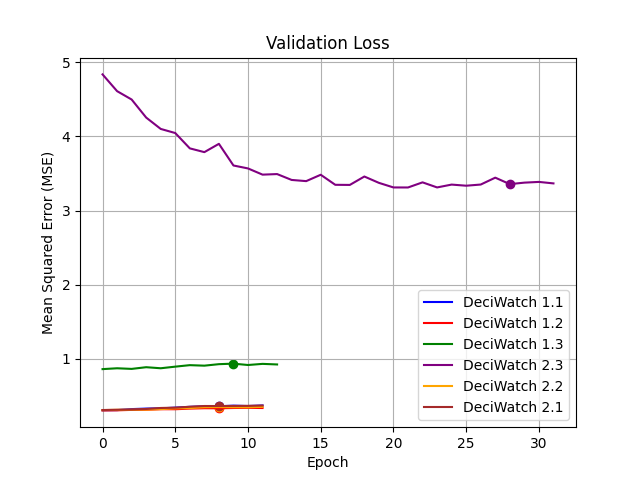
\includegraphics[width=0.32\textwidth]{./entities/finetuned/adapted/val_losses.png}
    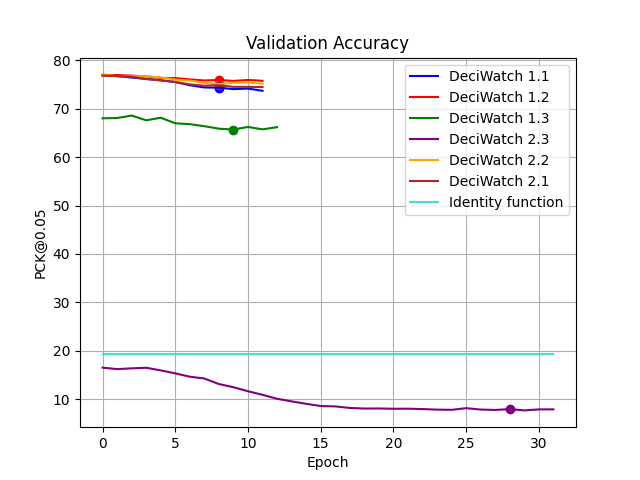
\includegraphics[width=0.32\textwidth]{./entities/finetuned/adapted/val_accs.png}
    \caption{Finetuning results of DeciWatch with regularization techniques.}
    \label{fig:finetune_res_2}
\end{figure}
As seen in Figure \ref{fig:finetune_res}, most of the DeciWatch methods would immediately overfit, as the validation loss increased while the training loss decreased, leading to the validation accuracy decreasing overtime. We performed further experiments, where we implemented various regularization techniques in hopes of this would lower the likelihood of the models overfitting. This was done by (1) freezing the whole network except for the very last fully-connected layer, which we reinitialized randomly, (2) added variance to the data by rotating each window throughout the training with a random degree in the range $[-45, 45]$, and (3) by applying weight decay with $\lambda = 0.001$.
\\
\\
By incorporating these regularization techniques we obtain the results visualized in Figure \ref{fig:finetune_res_2}. While the training loss doss generally decrease much slower than previously, the validation loss is still increasing and the validation PCK@0.2 accuracy is also decreasing, making the best setting of the models without these regularization methods perform either at the same level or an even better level than the models with regularization.


\subsection{Test Results}
\label{subsec:finetune_test_res}
\begin{table}[htbp]
    \begin{tabular}{c||ccc|ccc|ccc}
        \hline
        Accuracy metric & \multicolumn{3}{c}{PCK@0.05} & \multicolumn{3}{c}{PCK@0.1} & \multicolumn{3}{c}{PCK@0.2} \\
        \hline
        Mean threshold distance (px)* & \multicolumn{3}{c}{0.80} & \multicolumn{3}{c}{1.60} & \multicolumn{3}{c}{3.21} \\
        \hline
        Experiment & 1.1 & 1.2 & 1.3 & 1.1 & 1.2 & 1.3 & 1.1 & 1.2 & 1.3 \\
        \hline
        \hline
        Identity function & 19.4 & 19.4 & 19.4 & 66.1 & 66.1 & 66.1 & 85.2 & 85.2 & 85.2 \\
        3DConv & 49.7 & 52.3 & 53.1 & \textbf{95.7} & \textbf{95.7} & \textbf{95.8} & 99.2 & 99.3 & 99.3 \\
        DeciWatch & \textbf{76.6} & \textbf{76.7} & \textbf{68.1} & 94.4 & 94.3 & 87.3 & 99.2 & 99.2 & 96.1 \\
        bi-ConvLSTM - Model S & 37.8 & 34.9 & 39.0 & 91.8 & 92.1 & 92.2 & 99.4 & \textbf{99.7} & 99.2 \\
        bi-ConvLSTM - Model C & 35.9 & 39.0 & 38.5 & 93.1 & 93.6 & 92.6 & \textbf{99.8} & \textbf{99.7} & \textbf{99.7} \\
        \hline
    \end{tabular}
    \caption{Testing accuracies of the various developed models for shifting-scalar $s = 1$. All the accuracies are in percentage. *: The mean maximum distance between the predicted keypoint and corresponding ground truth keypoint for the prediction to count as being correct, measured in the heatmap coordinate system.}
    \label{tab:finetune_test_accs_1}
\end{table}

\begin{table}[htbp]
    \begin{tabular}{c||ccc|ccc|ccc}
        \hline
        Accuracy metric & \multicolumn{3}{c}{PCK@0.05} & \multicolumn{3}{c}{PCK@0.1} & \multicolumn{3}{c}{PCK@0.2} \\
        \hline
        Mean threshold distance (px)* & \multicolumn{3}{c}{0.80} & \multicolumn{3}{c}{1.60} & \multicolumn{3}{c}{3.21} \\
        \hline
        Experiment & 2.1 & 2.2 & 2.3 & 2.1 & 2.2 & 2.3 & 2.1 & 2.2 & 2.3 \\
        \hline
        \hline
        Identity function & 19.4 & 19.4 & 19.4 & 66.1 & 66.1 & 66.1 & 85.2 & 85.2 & 85.2 \\
        3DConv & 46.5 & 51.6 & \textbf{47.3} & \textbf{95.5} & \textbf{95.5} & \textbf{95.8} & 99.2 & 99.3 & 99.2 \\
        DeciWatch & \textbf{76.0} & \textbf{75.9} & 36.8 & 94.2 & 94.2 & 74.9 & 99.2 & 99.2 & 92.8 \\
        bi-ConvLSTM - Model S & 38.8 & 37.4 & 35.9 & 92.7 & 92.1 & 91.2 & 99.4 & \textbf{99.5} & 99.3 \\
        bi-ConvLSTM - Model C & 39.2 & 39.5 & 37.1 & 92.5 & 92.9 & 92.6 & \textbf{99.6} & 99.3 & \textbf{99.6} \\
        \hline
    \end{tabular}
    \caption{Testing accuracies of the various developed models for shifting-scalar $s = 2$. All the accuracies are in percentage. *: The mean maximum distance between the predicted keypoint and corresponding ground truth keypoint for the prediction to count as being correct, measured in the heatmap coordinate system.}
    \label{tab:finetune_test_accs_2}
\end{table}

\noindent We have in Table \ref{tab:finetune_test_accs_1} and Table \ref{tab:finetune_test_accs_2} illustrated the testing results of the epoch of each model that yielded the highest validation PCK@0.05 accuracy.
\\
\\
By comparing the two tables against each other we see, that the shifting-scalar only have a minor effect on the results of the models. Generally however, the models do perform the best with the noise-scalar $s = 1$.
\\
\\
Similarly to the pretraining stage, we also see here how 3DConv from experiment 2 performs better than 3DConv from experiment 1, however, this performance difference is now smaller than it was in the pretraining stage.
\\
\\
Further, for experiment 3 DeciWatch is not delivering great results, similarly to its results in the pretraining stage. For the other architectures, there do not seem to be any consistent pattern, as for some of them, experiment 3 yields the best results, whereas it for others yield the worst results.
\\
\\
Like in the pretraining stage, there does only seem to be a minor performance differences between the two architectures that are based on the bidirectional convolutional LSTM, making us further believe that our concern about the missing opportunity of bi-Conv LSTM Model S to prioritize a processing direction is only a minor problem.

\begin{table}[htbp]
    \begin{tabular}{c||ccc|ccc|ccc}
        \hline
        Accuracy metric & \multicolumn{3}{c}{PCK@0.05} & \multicolumn{3}{c}{PCK@0.1} & \multicolumn{3}{c}{PCK@0.2} \\
        \hline
        Mean threshold distance* & \multicolumn{3}{c}{0.87} & \multicolumn{3}{c}{1.77} & \multicolumn{3}{c}{3.55} \\
        \hline
        Experiment & 1.1 & 1.2 & 1.3 & 1.1 & 1.2 & 1.3 & 1.1 & 1.2 & 1.3 \\
        \hline
        \hline
        Identity function & 21.2 & 21.2 & 21.2 & 65.5 & 65.5 & 65.5 & 84.7 & 84.7 & 84.7 \\
        3DConv & 58.4 & 61.4 & 61.7 & \textbf{98.7} & \textbf{98.9} & \textbf{99.0} & \textbf{99.6} & \textbf{99.8} & \textbf{99.7} \\
        DeciWatch & \textbf{82.6} & \textbf{82.4} & \textbf{74.6} & 96.2 & 96.1 & 92.3 & 99.1 & 99.1 & 97.4 \\
        bi-ConvLSTM - Model S & 45.7 & 45.0 & 47.6 & 97.3 & 96.9 & 97.0 & \textbf{99.6} & \textbf{99.6} & 99.1 \\
        bi-ConvLSTM - Model C & 44.5 & 46.1 & 48.5 & 97.4 & 97.9 & 97.9 & 99.6 & 99.5 & 99.6 \\
        \hline
    \end{tabular}
    \caption{Testing accuracies of the various developed models for shifting-scalar $s = 1$ on the additional test video. All the accuracies are in percentage. *: The mean maximum distance between the predicted keypoint and corresponding ground truth keypoint for the prediction to count as being correct, using the units of the heatmap coordinates.}
    \label{tab:finetune_test_accs_3}
\end{table}

\begin{table}[htbp]
    \begin{tabular}{c||ccc|ccc|ccc}
        \hline
        Accuracy metric & \multicolumn{3}{c}{PCK@0.05} & \multicolumn{3}{c}{PCK@0.1} & \multicolumn{3}{c}{PCK@0.2} \\
        \hline
        Mean threshold distance* & \multicolumn{3}{c}{0.87} & \multicolumn{3}{c}{1.77} & \multicolumn{3}{c}{3.55} \\
        \hline
        Experiment & 2.1 & 2.2 & 2.3 & 2.1 & 2.2 & 2.3 & 2.1 & 2.2 & 2.3 \\
        \hline
        \hline
        Identity function & 21.2 & 21.2 & 21.2 & 65.5 & 65.5 & 65.5 & 84.7 & 84.7 & 84.7 \\
        3DConv & 56.2 & 60.0 & \textbf{56.6} & \textbf{98.9} & \textbf{98.8} & \textbf{98.8} & \textbf{99.7} & \textbf{99.7} & \textbf{99.7} \\
        DeciWatch & \textbf{81.6} & \textbf{81.8} & 37.5 & 96.0 & 96.0 & 73.3 & 99.1 & 99.1 & 90.7 \\
        bi-ConvLSTM - Model S & 44.8 & 46.2 & 45.0 & 96.9 & 95.9 & 97.1 & 99.5 & 99.6 & 99.5 \\
        bi-ConvLSTM - Model C & 45.9 & 47.9 & 46.7 & 96.7 & 97.1 & 98.1 & 99.6 & 99.4 & 99.6 \\
        \hline
    \end{tabular}
    \caption{Testing accuracies of the various developed models for shifting-scalar $s = 2$ on the additional test video. All the accuracies are in percentage. *: The mean maximum distance between the predicted keypoint and corresponding ground truth keypoint for the prediction to count as being correct, using the units of the heatmap coordinates.}
    \label{tab:finetune_test_accs_4}
\end{table}

\noindent One might argue, that our way of splitting the finetuning dataset into a validation and test dataset might introduce some bias, as the two datasets have overlapping videos and thus videos of the same person that might have some unique movement. To further minimize the likelihood of a biased evaluation of the models, we have in Table \ref{tab:finetune_test_accs_3} and Table \ref{tab:finetune_test_accs_4} tested the models on the longest video of the dataset, consisting of 754 overlapping windows, which was not used at all in any of the three datasubsets. By comparing these tables against Table \ref{tab:finetune_test_accs_1} and \ref{tab:finetune_test_accs_2} we can clearly see, that the models are performing similarly, if not actually better, than how they did previously, hence why we would argue, that there are no indication of the first test evaluation being biased. However, we have to note, that the evaluation in Table \ref{tab:finetune_test_accs_3} and Table \ref{tab:finetune_test_accs_4} do contain some bias, as the evaluation is of a single person who might have some easily predictable movements.
\\
\\
\begin{table}[htbp]
    \begin{adjustbox}{center}
        \begin{tabular}{c||ccc|ccc|ccc|ccc|c}
            \hline
            & \multicolumn{3}{c}{3DConv} & \multicolumn{3}{c}{DeciWatch} & \multicolumn{3}{c}{\begin{tabular}[c]{@{}c@{}}bi-ConvLSTM\\ Model S\end{tabular}} & \multicolumn{3}{c}{\begin{tabular}[c]{@{}c@{}}bi-ConvLSTM\\ Model C\end{tabular}} & Total \\ 
            \hline
            Experiment & 1.1 & 1.2 & 1.3 & 1.1 & 1.2 & 1.3 & 1.1 & 1.2 & 1.3 & 1.1 & 1.2 & 1.3 & \\
            \hline
            \hline
            Nose & 95.5 & 97.6 & 95.7 & 94.9 & 94.9 & 88.5 & 93.5 & 89.7 & 95.4 & 93.4 & 88.8 & 90.9 & 93.2 \\
            Ear & 96.5 & 96.7 & 96.8 & 95.5 & 95.5 & 88.6 & 94.3 & 91.9 & 94.2 & 96.3 & 95.6 & 96.1 & 94.8 \\
            Shoulder & 95.6 & 97.4 & 97.1 & 95.4 & 95.4 & 88.4 & 91.2 & 90.6 & 87.2 & 91.9 & 95.1 & 92.9 & 93.2 \\
            Elbow & 97.6 & 97.2 & 97.5 & 94.5 & 94.6 & 86.5 & 93.2 & 93.7 & 94.9 & 95.1 & 96.7 & 95.2 & 94.7 \\
            Wrist & 96.4 & 96.4 & 96.3 & 93.9 & 93.9 & 85.8 & 94.2 & 92.7 & 94.1 & 94.5 & 93.2 & 94.3 & 93.8 \\
            Pinky & 86.6 & 85.4 & 85.4 & 92.5 & 92.2 & 84.0 & 84.5 & 86.5 & 86.6 & 83.4 & 88.4 & 87.0 & 86.9 \\
            Index finger & 92.7 & 92.5 & 93.1 & 92.2 & 92.1 & 84.3 & 90.3 & 89.1 & 88.2 & 89.9 & 92.3 & 92.1 & 90.7 \\
            Thumb & 91.6 & 91.0 & 91.4 & 92.8 & 92.7 & 84.5 & 81.0 & 89.3 & 84.9 & 89.6 & 85.5 & 86.9 & 88.4 \\
            Hip & 99.4 & 99.0 & 99.8 & 96.4 & 96.4 & 89.9 & 92.5 & 96.5 & 98.0 & 94.6 & 97.7 & 96.1 & 96.4 \\
            Knee & 97.7 & 98.1 & 98.4 & 95.0 & 95.0 & 88.4 & 96.1 & 92.5 & 96.5 & 96.0 & 93.9 & 93.6 & 95.1 \\
            Ankle & 98.6 & 98.4 & 99.1 & 95.0 & 95.0 & 87.6 & 94.3 & 93.6 & 96.0 & 97.2 & 98.1 & 94.3 & 95.6 \\
            Heel & 98.6 & 98.1 & 98.5 & 95.2 & 95.1 & 86.2 & 94.2 & 93.4 & 94.9 & 92.5 & 92.6 & 93.0 & 94.4 \\
            Toes & 97.2 & 97.5 & 98.0 & 94.2 & 94.0 & 86.8 & 94.9 & 95.3 & 95.5 & 93.8 & 95.7 & 94.4 & 94.8 \\
            \hline
            Total & 95.7 & 95.7 & 95.8 & 94.4 & 94.3 & 87.3 & 91.8 & 92.1 & 92.2 & 93.1 & 93.6 & 92.6 & \\
            \hline
        \end{tabular}
    \end{adjustbox}
    \caption{Keypoint-specific testing PCK@0.1-accuracies of the various models for shifting-scalar $s = 1$. All the accuracies are in percentage.}
    \label{tab:finetune_kpts_test_accs_1_1}
\end{table}

\begin{table}[htbp]
    \begin{adjustbox}{center}
        \begin{tabular}{c||ccc|ccc|ccc|ccc|c}
            \hline
            & \multicolumn{3}{c}{3DConv} & \multicolumn{3}{c}{DeciWatch} & \multicolumn{3}{c}{\begin{tabular}[c]{@{}c@{}}bi-ConvLSTM\\ Model S\end{tabular}} & \multicolumn{3}{c}{\begin{tabular}[c]{@{}c@{}}bi-ConvLSTM\\ Model C\end{tabular}} & Total \\ 
            \hline
            Experiment & 1.1 & 1.2 & 1.3 & 1.1 & 1.2 & 1.3 & 1.1 & 1.2 & 1.3 & 1.1 & 1.2 & 1.3 & \\
            \hline
            \hline
            Nose & 95.6 & 97.0 & 95.6 & 94.1 & 94.3 & 80.8 & 90.9 & 89.6 & 93.2 & 88.1 & 91.1 & 90.8 & 91.76 \\
            Ear & 96.8 & 95.7 & 96.9 & 93.3 & 93.4 & 80.8 & 94.2 & 92.7 & 92.6 & 91.9 & 93.2 & 94.9 & 93.0 \\
            Shoulder & 95.1 & 97.1 & 95.7 & 95.3 & 95.4 & 77.5 & 93.5 & 93.4 & 90.1 & 90.0 & 97.7 & 95.6 & 93.0 \\
            Elbow & 97.2 & 97.1 & 97.5 & 94.4 & 94.5 & 72.0 & 96.0 & 96.7 & 90.9 & 97.1 & 97.0 & 94.7 & 93.8 \\
            Wrist & 96.4 & 96.5 & 96.6 & 93.8 & 93.8 & 77.4 & 89.2 & 93.8 & 91.9 & 93.2 & 94.3 & 9.33 & 85.5 \\
            Pinky & 85.0 & 85.3 & 87.0 & 92.3 & 92.4 & 66.1 & 84.5 & 82.6 & 84.0 & 87.4 & 83.6 & 89.7 & 85.0 \\
            Index finger & 93.1 & 92.8 & 93.0 & 92.5 & 92.5 & 65.3 & 92.7 & 89.9 & 92.4 & 92.1 & 88.0 & 91.4 & 89.6 \\
            Thumb & 91.1 & 90.8 & 91.6 & 93.0 & 92.9 & 71.4 & 85.3 & 83.5 & 81.1 & 82.6 & 84.6 & 88.9 & 86.4 \\
            Hip & 99.3 & 98.8 & 99.6 & 96.3 & 96.4 & 78.6 & 97.1 & 96.2 & 96.8 & 97.8 & 97.4 & 84.5 & 94.9 \\
            Knee & 97.6 & 97.8 & 97.9 & 95.1 & 95.0 & 77.9 & 94.9 & 93.3 & 91.3 & 95.9 & 98.4 & 97.5 & 94.4 \\
            Ankle & 98.6 & 98.5 & 99.3 & 94.5 & 94.6 & 79.3 & 96.2 & 96.0 & 93.8 & 98.5 & 96.8 & 96.2 & 95.2 \\
            Heel & 98.2 & 97.8 & 98.8 & 95.1 & 95.0 & 78.5 & 93.7 & 93.0 & 93.2 & 93.0 & 91.3 & 92.8 & 93.4 \\
            Toes & 97.4 & 97.4 & 97.8 & 94.0 & 94.0 & 73.1 & 95.1 & 96.8 & 93.5 & 92.7 & 93.7 & 93.7 & 93.3 \\
            \hline
            Total & 95.5 & 95.5 & 95.8 & 94.2 & 94.2 & 74.9 & 92.7 & 92.1 & 91.2 & 92.5 & 92.9 & 92.6 & \\
            \hline
        \end{tabular}
    \end{adjustbox}
    \caption{Keypoint-specific testing PCK@0.1-accuracies of the various models for shifting-scalar $s = 2$. All the accuracies are in percentage.}
    \label{tab:finetune_kpts_test_accs_1_2}
\end{table}

\noindent We have in Table \ref{tab:finetune_kpts_test_accs_1_1} and Table \ref{tab:finetune_kpts_test_accs_1_2} illustrated the keypoint specific PCK@$0.1$ testing accuracies of the models. For the equivalent tables of PCK$@0.05$ and PCK$@0.2$ see Table \ref{tab:finetune_kpts_test_accs_05_1}-\ref{tab:finetune_kpts_test_accs_2_2} in the appendix. By comparing these two tables to the equivalent tables from section \ref{subsec:pretrain_train_val_res} we see, that the most difficult keypoints are no longer the wrists and ankles, but generally are instead the pinkies, the index fingers and the thumbs, on which the models generally performs much worse than on the remaining keypoints.
\\
\\
For some illustrations of the predictions of the best setup of each model based on Table \ref{tab:finetune_test_accs_1} and Table \ref{tab:finetune_test_accs_2}, see Figure \ref{fig:predictions} in the appendix.

\subsection{Technical Details}
\label{sec:finetune_tech_details}
All models were trained and evaluated using an 8GB NVIDIA GTX 1070 and an Intel Core i7-4790K @ 4.00GHz. All models were implemented in Python version 3.9.9 using PyTorch 2.0.0. 3DConv took about 1.5 minutes per epoch, DeciWatch about 2 minutes per epoch, and the two bidirectional convolutional LSTMs took about 2.5 minutes per epoch each.

\end{document}